\nnarticleheader{The Fermi Paradox: Are We Alone?}{Matthew Wang, Haverford '21}

\noindent
\textbf{Are We Alone?}

Once in a while, this simple question might jump into your head, creating a wave of mystery and awe. The fact remains that the observable universe is about 93 billion light-years in diameter, yet why haven’t humans found any trace of alien, bacterial, or any carbon-based life forms?

This paradox is what we humans know as The Fermi Paradox. Enrico Fermi had the same question, as the evidence that supports life through the galaxy is indeed optimistic. Billions of Earth-like planets and sun-like stars roam our universe, each has the capability to foster life and more. A closely related question, the Drake Equation, is a systematic means to evaluate the probabilities involved in the existence of alien life. It takes into account the details and intricacies of a galaxy, solar system, and planetary formation. So far, the wait continues for the day humans learn of alien-life. Whether it’s deep inside of Europa (Jupiter’s moon, as shown below), or the Andromeda galaxy; humans still wait.

\renewcommand{\thefigure}{1}
\begin{figure}[h]
  \begin{center}
    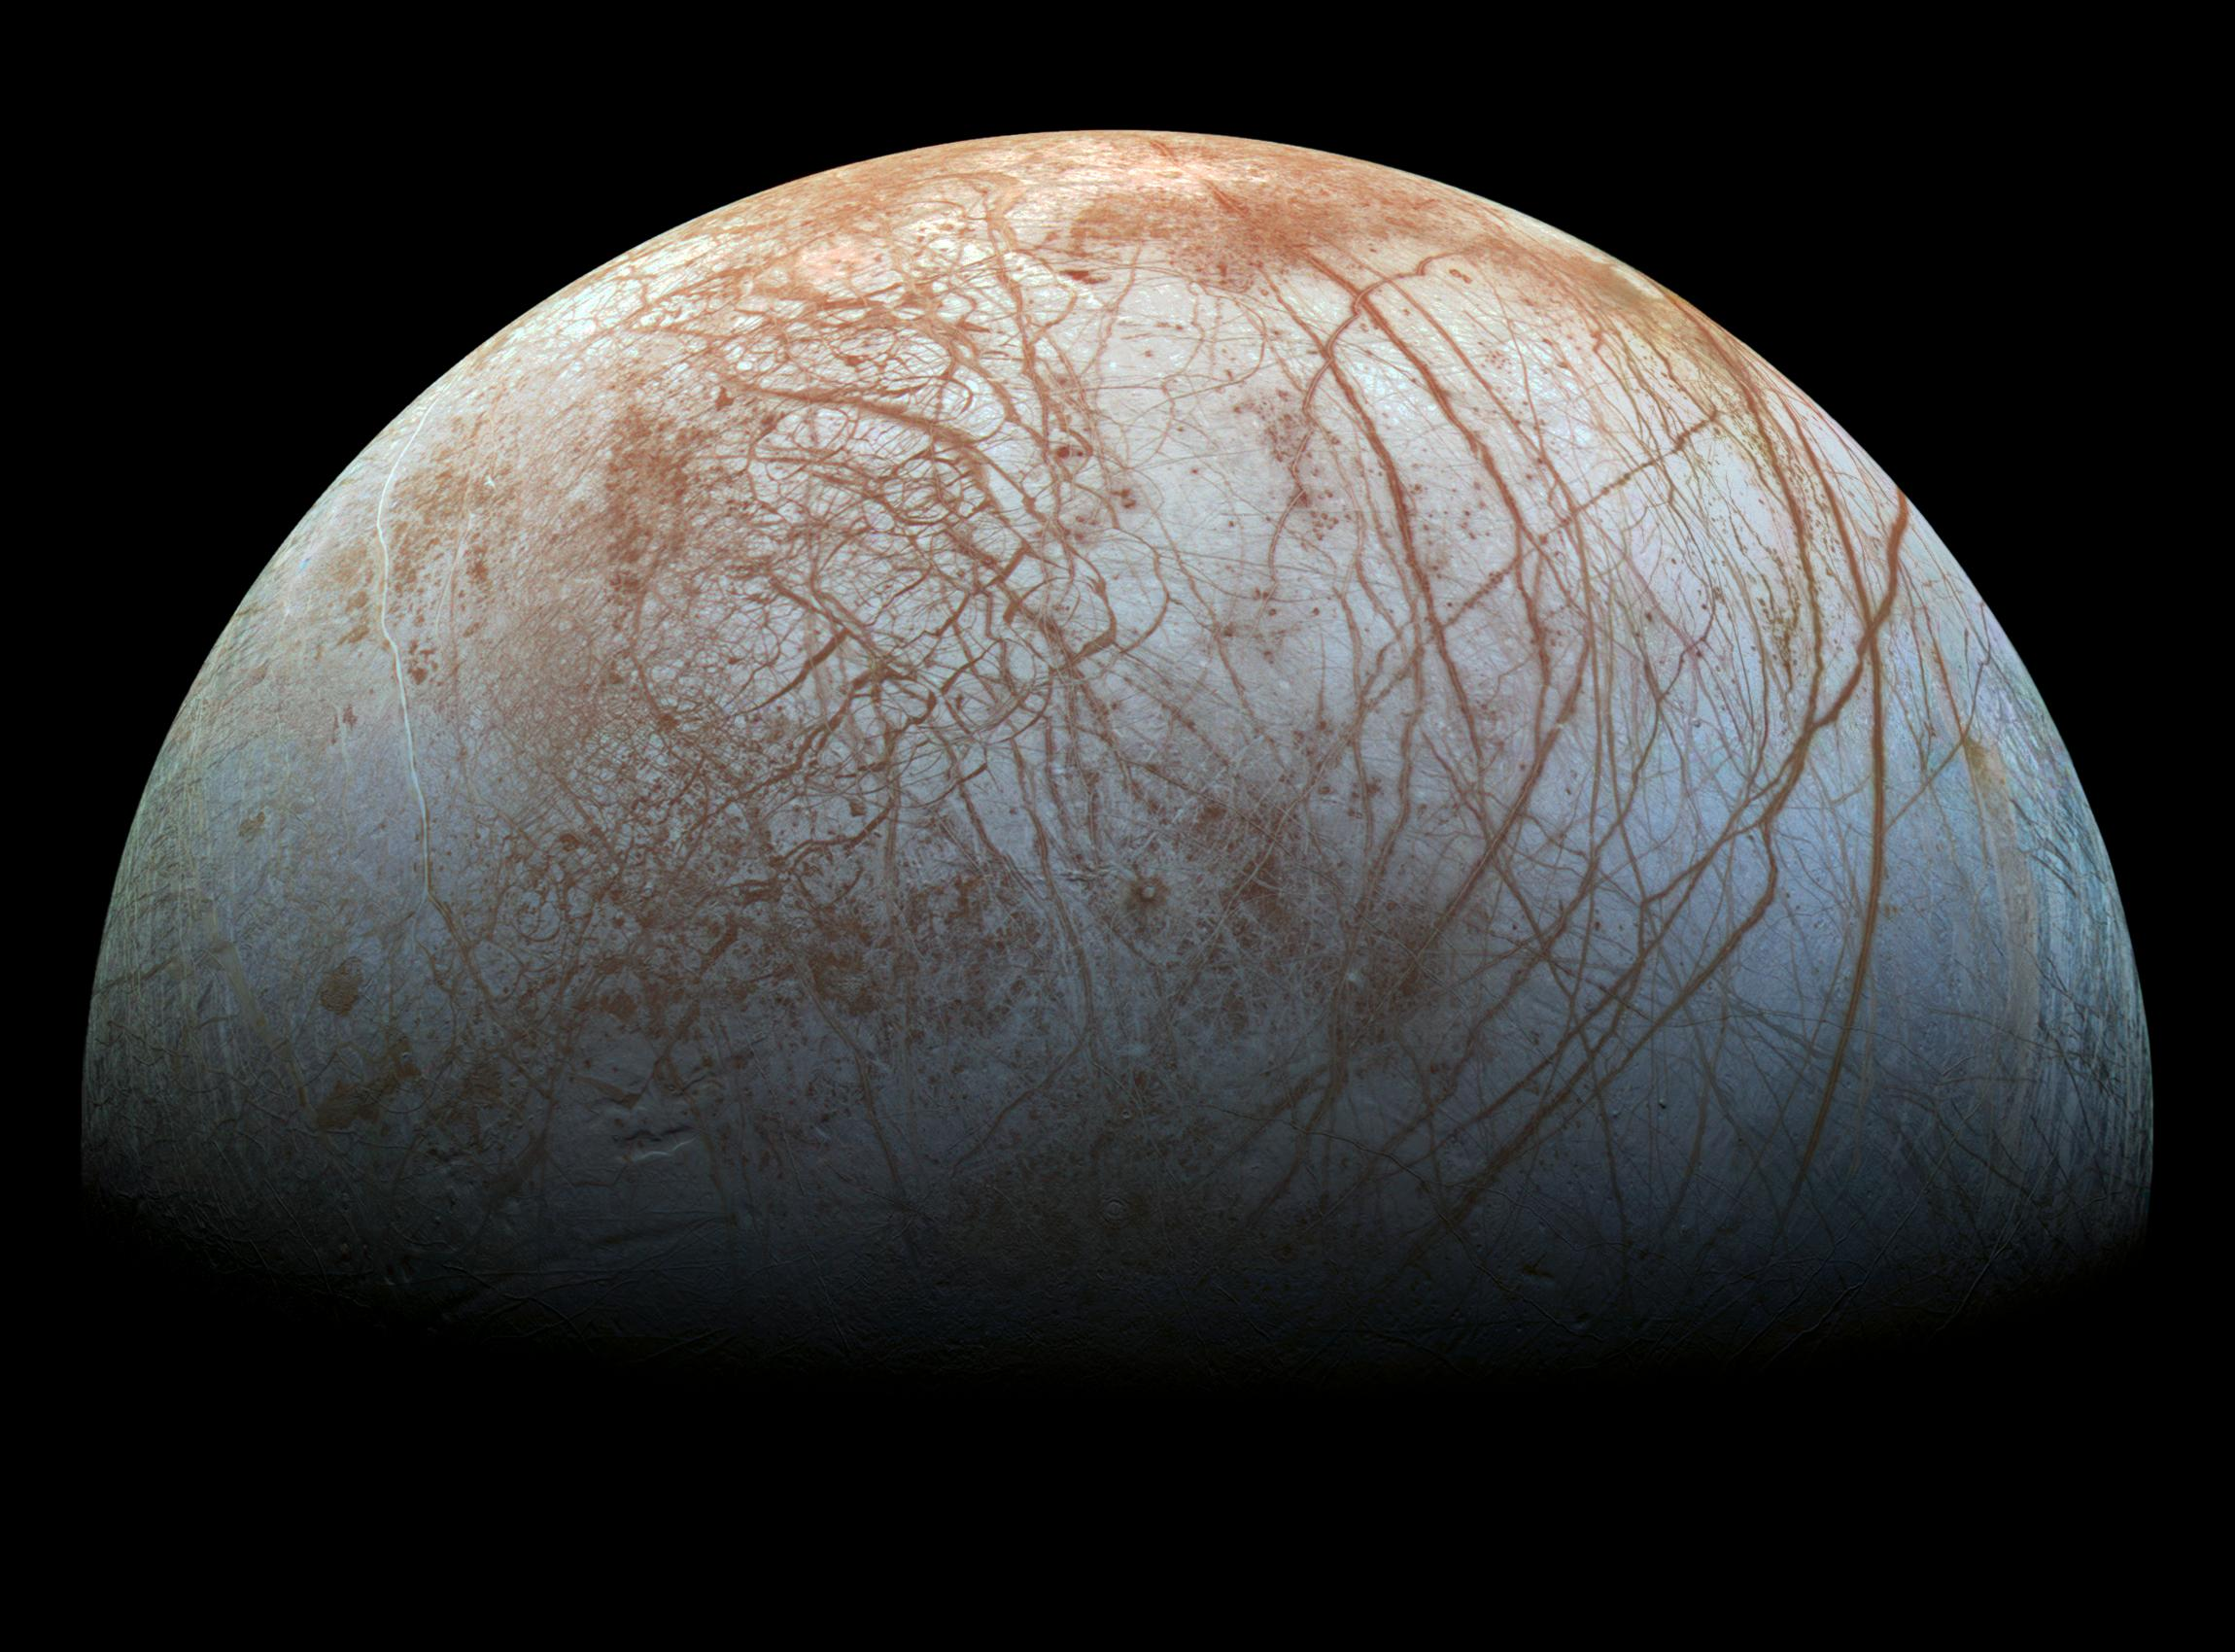
\includegraphics[width=7cm]{wang_image1}
  \end{center}
  \caption{Europa, a moon of Jupiter.}
  \label{fig:1}
\end{figure}

\noindent
\textbf{Possible Explanations}

According to the Kardeshev Scale (a scale that measures a civilization’s level of power, down below), humans have yet to reach stage one. Each level corresponds to a civilization’s power occupancy. The list is as follows: full planetary, solar system, galactical, and universal control. Yet, if an alien civilization were to have advanced through these levels, wouldn’t humans have found signals of life? 

\begin{figure}[htp]
    \centering
    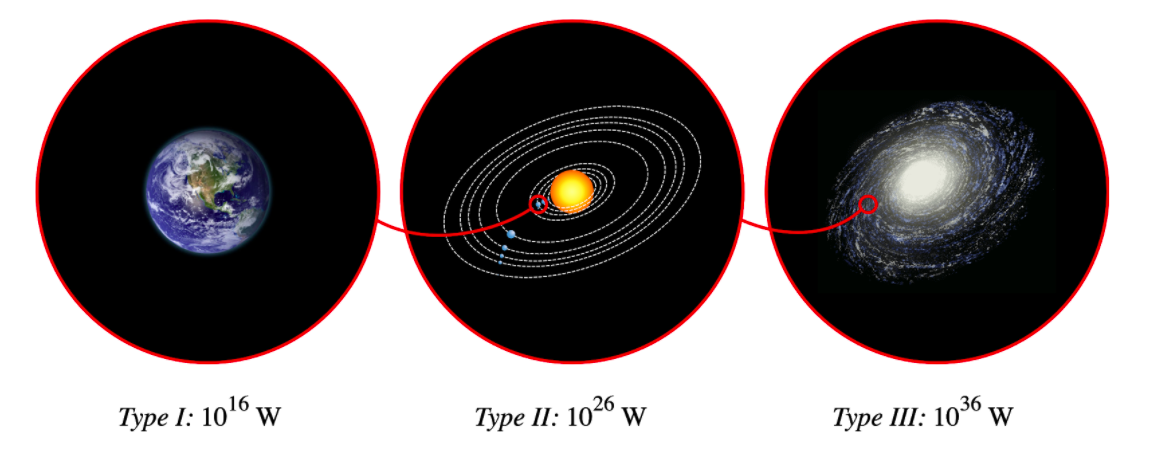
\includegraphics[width=7cm]{wang_image2}
    \caption{The Kardeshec Scale}
    \label{fig:2}
\end{figure}

\pagebreak

Known as the Great Filter, there are two widely accepted answers. Life is Rare! Extremely rare. Humans would not have existed if it weren’t for luck. It’s possible that human thought is simply so rare it’s only occurred once. Another answer lies in the fact that intelligent thought always destroys itself. Through technological wars, these intelligent life forms always kill themselves before reaching higher levels of civilization. Now a new question arises. Have we crossed this great filter or have we yet to destroy ourselves? As Nuclear war seems like a possibility, the Anthropocene may be nearing the end. It may be up to us humans to pass this filter.
